\documentclass[3p]{elsarticle}
\usepackage{rotating} 
\graphicspath{ {./figures/} }
\usepackage{hyperref}
\usepackage{float}
\usepackage{verbatim} %comments
\usepackage{apalike}
\restylefloat{figure}
\floatstyle{plaintop} %table caption at top
\restylefloat{table}
\usepackage{enumitem} % For custom list labels
\usepackage{amsmath, amssymb}  % Required for \boldsymbol
\usepackage{graphicx}
\usepackage{algorithm}
\usepackage{algpseudocode}
\usepackage{booktabs}
\usepackage{caption}
\captionsetup[figure]{labelformat=default, labelsep=period, name=Fig.}
\newcommand{\Indent}{\State\hspace{\algorithmicindent}}
\newcommand{\Indentx}{\Statex\hspace{\algorithmicindent}}

\begin{document}
\begin{frontmatter}

\title{\textbf{PLOJF: Polar Lights Optimization with Jumping Historical Search and Fitness-Diversity Balancing}}

\begin{abstract}

\end{abstract}

\begin{keyword}

\end{keyword}

\end{frontmatter}

\section{The Proposed PLOJF Algorithm}
In this section, we introduce the proposed PLOJF algorithm. By integrating a Jumping Historical Search strategy and a Fitness-Diversity Balanced (FDB) selection mechanism, PLOJF enhances the search efficiency and solution precision of the original PLO algorithm.

\subsection{Polar Lights Optimization}
Polar Lights Optimization (PLO) is a metaheuristic inspired by the auroral phenomena observed near the Earth's poles. It balances exploration and exploitation through three coordinated mechanisms: (i) a gyration motion that provides local exploitation, (ii) an auroral oval walk guided by a Lévy flight to encourage global exploration, and (iii) a particle-collision–based refinement that adjusts solutions at the dimension level. An adaptive weighting scheme modulates the influence of the local and global components over the course of the search, enabling PLO to shift focus as needed.

Gyration motion is motivated by the trajectories of high-energy charged particles moving in a magnetic field. Let \(q\) denote the particle charge, \(v\) its velocity, \(B\) the magnetic field, and \(m\) the mass. A simplified first-order model for the velocity dynamics is
\[ m\frac{dv}{dt} = q\,v\,B \qquad(1) \]
To account for atmospheric damping, a factor \(\alpha\) is introduced, yielding
\[ m\frac{dv}{dt} = q\,v\,B - \alpha v \qquad(2) \]
Solving (2) gives
\[ v(t) = C\,e^{\frac{qB-\alpha}{m}t} \qquad(3) \]
where \(C\) is a constant of integration. In the original setting, parameters are typically normalized with \(C=q=B=1\), \(m=100\), \(\alpha\in[1,1.5]\), and the time variable \(t\) is tied to the number of function evaluations.

To strengthen global exploration, PLO employs an auroral oval walk guided by a Lévy flight and the population mean. For individual \(i\), the exploratory step is
\[ Ao = \mathrm{Levy}(\mathrm{dim})\times(X_{\mathrm{avg}} - X_i) + LB + r_1\times\frac{UB - LB}{2} \qquad(4) \]
where \(\mathrm{Levy}(\cdot)\) denotes a Lévy-flight–based perturbation, \(X_{\mathrm{avg}}\) is the population mean, \(LB\) and \(UB\) are the lower and upper bounds, and \(r_1\in[0,1]\).

Local and global moves are fused through an adaptive update rule
\[ X_i^{\mathrm{new}} = X_i + r_2\times\bigl(w_1\,v(t) + w_2\,Ao\bigr) \qquad(5) \]
where \(r_2\in[0,1]\) scales the step size, and \(w_1\) and \(w_2\) are time-varying weights defined as
\[ w_1 = \frac{2}{1 + e^{-2\left(\tfrac{t}{T}\right)^{4}}} - 1 \qquad(6) \]
\[ w_2 = e^{-\left(\tfrac{t}{T}\right)^{3}} \qquad(7) \]
Here, \(t\) is the current number of function evaluations and \(T\) is the predefined maximum.

Finally, PLO incorporates a dimension-wise refinement inspired by particle collisions in the solar wind:
\[ X_{i,j}^{\mathrm{new}} = X_{i,j} + \sin\!\bigl(r_3\,\pi\bigr)\times\bigl(X_{i,j} - X_{a,j}\bigr),\quad r_4 < K\ \text{ and }\ r_5 < 0.05 \qquad(8) \]
where \(r_3, r_4, r_5\sim\mathcal{U}(0,1)\), \(K\) is a trigger threshold, and \(X_a\) is a randomly selected peer. This refinement is applied sparingly across iterations, serving as a lightweight local search to polish candidate solutions.

\subsection{Limitations of PLO and Motivation}
While PLO provides a principled coupling of local exploitation (gyration), global exploration (auroral oval walk), and occasional dimension-wise refinement, its baseline dynamics can still exhibit two limiting behaviors on complex, multimodal landscapes.

First, PLO is prone to diversity erosion as the run progresses. As the population mean \(X_{\mathrm{avg}}\) concentrates and the adaptive weights emphasize exploitation, individuals increasingly crowd the current basins of attraction. Because the exploratory step in (4) is anchored to \(X_{\mathrm{avg}}\), and the refinement in (8) is applied sparingly, underperforming individuals may lack sufficient impetus to escape entrenched regions, risking premature convergence. An effective diversification mechanism should therefore provide targeted, history-informed perturbations that relocate poor performers to novel regions without disrupting promising trajectories.

Second, PLO typically relies on greedy, one-to-one replacement, admitting an offspring only if it immediately improves fitness. This myopic policy can discard candidates that, despite having slightly worse fitness, contribute valuable spatial diversity (for example, by residing far from the incumbent best). When the search stalls, such a policy accelerates collapse around suboptimal attractors and reduces the algorithm's long-term exploratory capacity. A more robust survivor selection should, at least under stagnation, account for both quality and spatial contribution.

These observations motivate two complementary enhancements. To counter diversity loss, we introduce a Jumping Historical Search (JHS) strategy that leverages an archive of recently replaced parents to construct differential, event-driven jumps for underperforming individuals, synergistically augmenting the exploratory move in (4). To mitigate myopic selection, we adopt a Fitness–Diversity Balanced (FDB) survivor selection that, when stagnation is detected, merges parents and offspring, preserves an elite set by pure fitness, and fills the remaining slots using a score that balances normalized fitness with a diversity component measured via distance to the current best. The following subsections detail JHS and FDB and how they integrate with PLO's operators.

\subsection{Jumping Historical Search(JHS)}
To counter diversity loss without disrupting promising trajectories, we employ an event-driven Jumping Historical Search (JHS). An external archive \(A\) stores recently replaced parents. For a small fraction of underperforming individuals (bottom \(q\) of the population), and only within a short window after an FDB event, JHS perturbs the exploratory candidate by a history-informed differential jump. Specifically, letting \(X_{\!\text{arch}}\in A\) be a randomly selected archived parent and \(\eta>0\) a small magnitude, we form
\[ \Delta = \eta\,\bigl(X_i - X_{\!\text{arch}}\bigr) \qquad(9) \]
and orthogonalize it against the current exploitation direction \(H\) to avoid fighting the intensification drive:
\[ \Delta \leftarrow \Delta - \frac{\langle \Delta, H \rangle}{\lVert H \rVert_2^2 + \varepsilon}\,H \qquad(10) \]
after which the exploratory move becomes
\[ X_{\mathrm{cand}} = X_{\mathrm{explore}} + \Delta \qquad(11) \]
Here, \(H\) is the hybrid guidance combining mean-, personal-best-, global-best-, and partner-driven components used in the baseline generator, and \(\varepsilon>0\) safeguards against division by zero. JHS is applied with a small probability to eligible individuals during a limited number of generations following an FDB trigger, providing targeted diversification precisely when stagnation is detected.

\subsection{Fitness-Diversity Balanced (FDB) Selection}
To mitigate myopic replacement and restore exploratory capacity under stagnation, we adopt a Fitness–Diversity Balanced (FDB) survivor selection. When triggered, parents and offspring are merged, and survivors are chosen in two phases. First, an elite set comprising roughly half the population is selected purely by fitness. Second, the remaining survivors are chosen by minimizing a composite score that balances normalized fitness and spatial diversity (diversity implemented as the Euclidean distance to the current best in the combined pool):
\[ \mathrm{FDB\_score}(x) = \mathrm{norm}\bigl(f(x)\bigr) + \mathrm{norm}\bigl(\,\|x - x^{\star}\|_2\,\bigr) \qquad(12) \]
This scheme preserves high-quality solutions while deliberately retaining individuals far from the current incumbent, preventing rapid collapse around a single basin and improving coverage of the search space. In our implementation, FDB is considered only after an initial portion of the budget has elapsed and when both low improvement and low diversity are detected; after an FDB event, a short cooldown is enforced and an event window activates JHS for the next few generations, coupling selection and diversification.

\subsection{Operational Procedure of PLOJF}
The proposed PLOJF enhances the original PLO by integrating the two strategies previously described: Jumping Historical Search (JHS) and Fitness–Diversity Balanced (FDB) selection. JHS provides targeted, event-driven diversification for underperforming individuals via archive-based differential jumps (9)–(11), while FDB replaces myopic greedy replacement with an adaptive, two-phase survivor selection that balances fitness and diversity (12). Their integration follows a detection-and-response cycle: when stagnation and low diversity are detected, FDB is triggered and a short window activates JHS to diversify the subsequent generations.

The complete operational flow is outlined in Algorithm 1.

\begin{figure}[h]
\centering
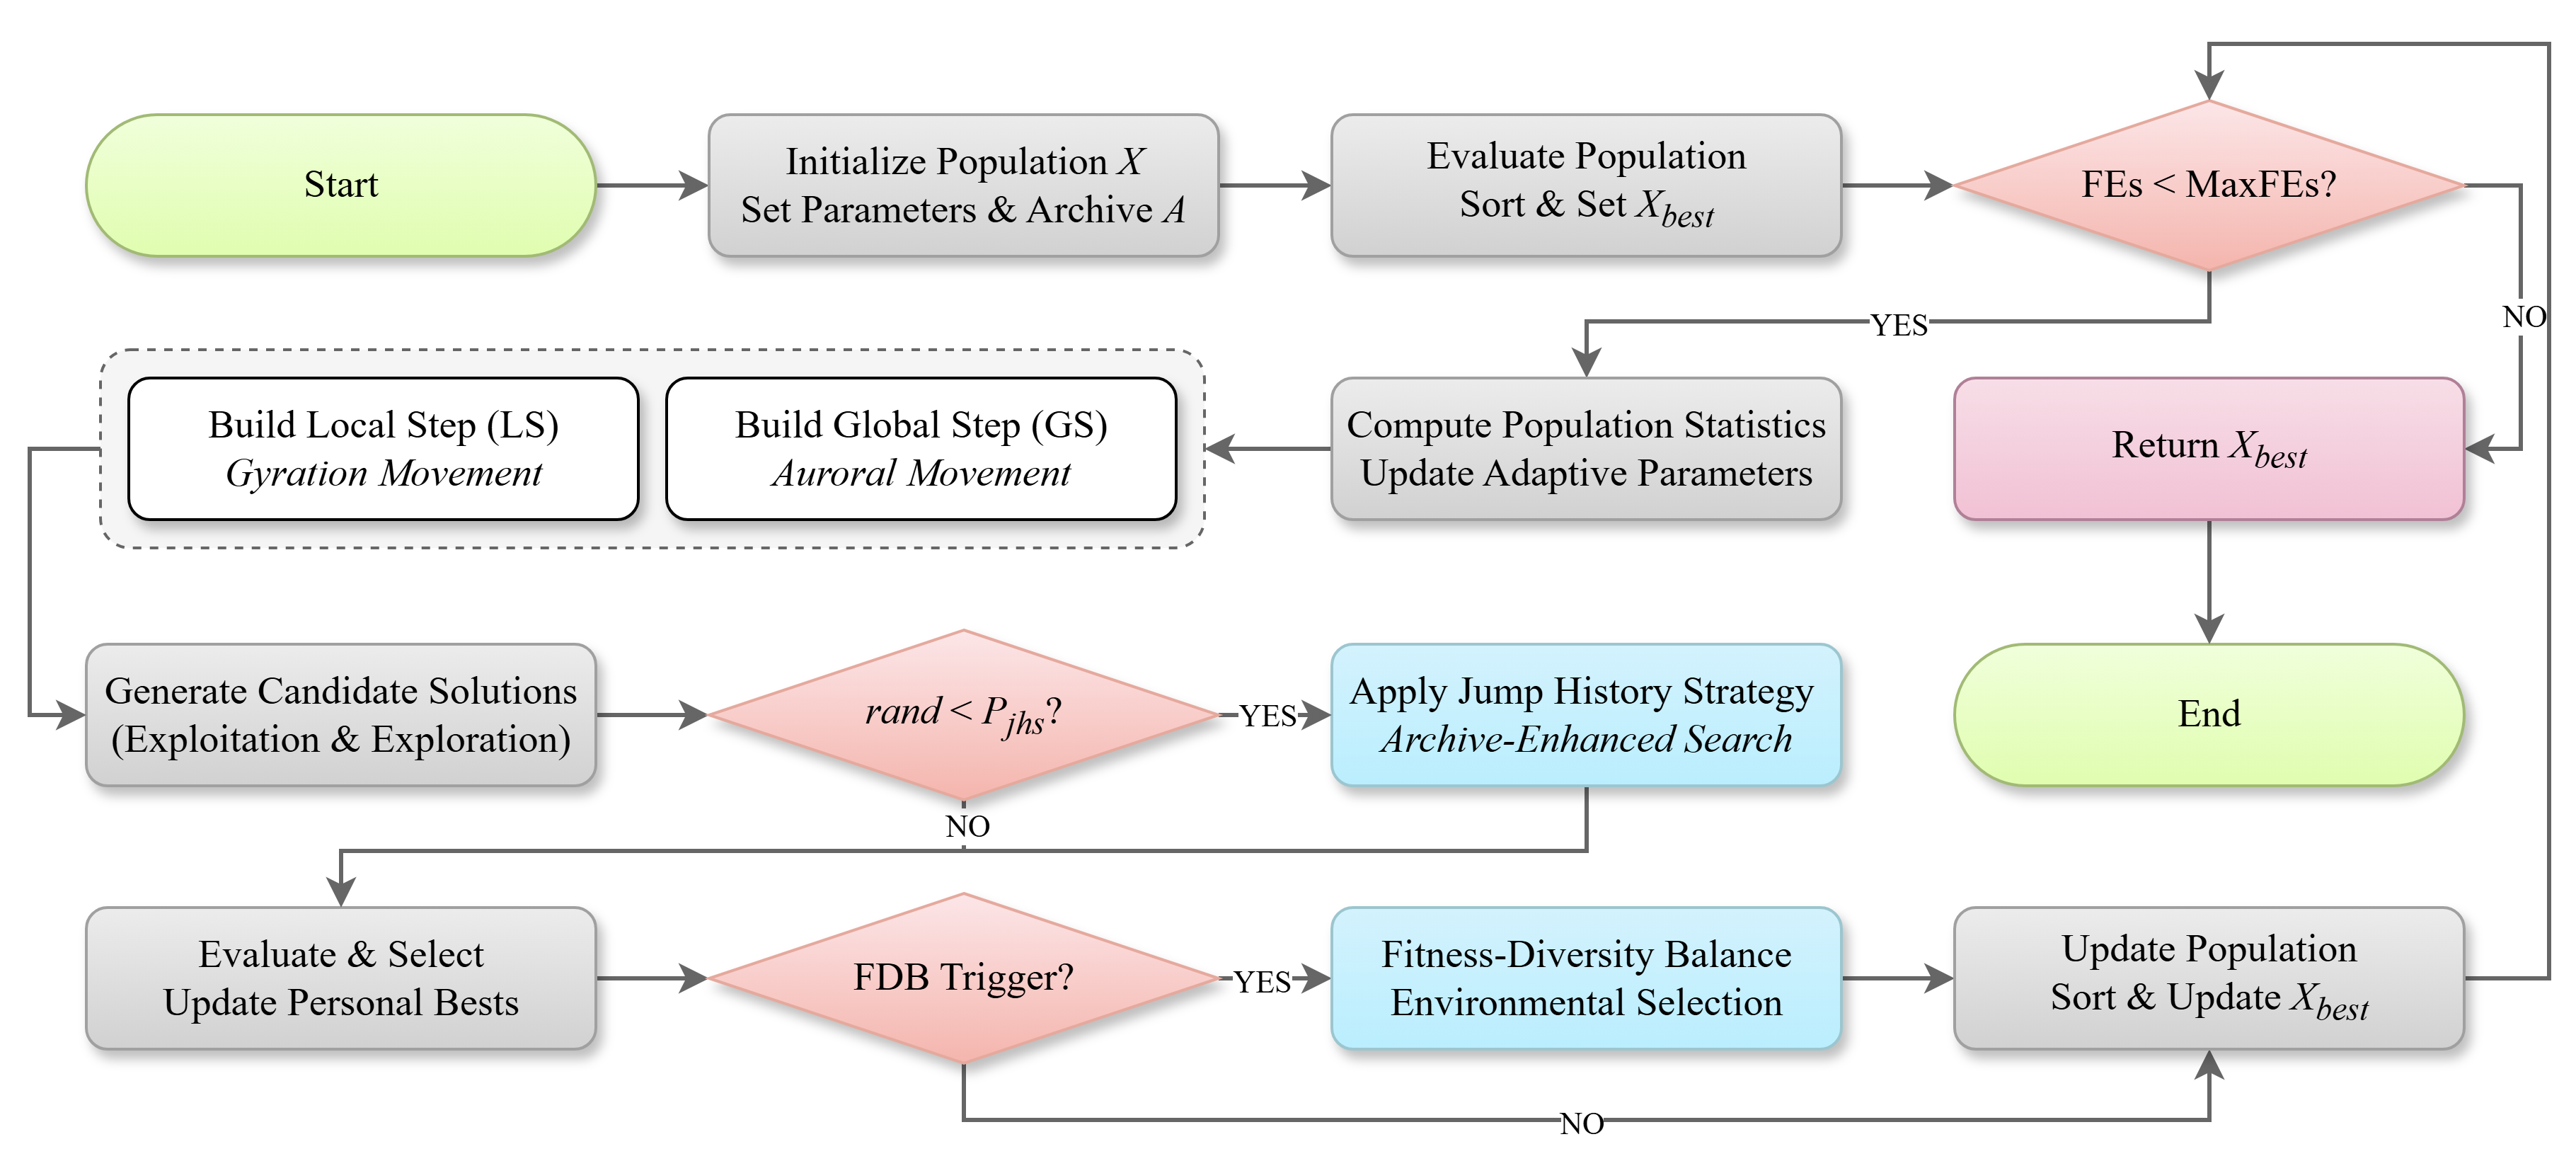
\includegraphics[width=0.8\textwidth]{PLOJF-flowchart}
\caption{PLOJF flowchart.}
\label{fig:flowchart}
\end{figure}

\begin{algorithm}
\caption{PLOJF Operational Procedure}
\label{alg:plojf}
\begin{algorithmic}[1]
\State \textbf{Input:} $N$, $MaxFEs$, $\mathrm{dim}$, $LB$, $UB$, objective $f$
\State \textbf{Output:} Best solution $X_{best}$
\State Initialize population $X\sim\mathcal{U}(LB,UB)$; evaluate $F$; sort; set $X_{best}$
\State Initialize personal bests $Pbest\leftarrow X$; archive $A\leftarrow\emptyset$; set adaptation and trigger parameters
\While{$FEs < MaxFEs$}
    \State Compute $X_{avg}$, adaptive weights $w_1$, $w_2$, success rate and scale; estimate diversity
    \State Derive probabilities $p_{\mathrm{explore}}$, $p_{\mathrm{cauchy}}$ and gain $g_s$; mark bottom-$q$ individuals
    \For{$i=1$ to $N$}
        \State Build local step $LS$ (gyration) and global step $GS$ (auroral) using population statistics
        \State Select partner (early split vs. later random in half); form hybrid guidance $H$
        \State Generate two candidates: $\mathrm{cand}_1$ (exploit) and $\mathrm{cand}_2$ (explore)
        \If{JHS window active and $i$ is bottom-$q$ and $A\neq\emptyset$ and $\mathrm{rand}<p_A$}
            \State Pick $X_{\!\text{arch}}\in A$; compute $\Delta=\eta\,(X_i-X_{\!\text{arch}})$; orthogonalize $\Delta$ to $H$ per (10)
            \State Update $\mathrm{cand}_2 \leftarrow \mathrm{cand}_2 + \Delta$ \hfill
        \EndIf
        \If{$\mathrm{rand} < p_{\mathrm{cauchy}}$} \State Apply Cauchy jump to $\mathrm{cand}_2$ around $X_i$ and $X_{best}$ \EndIf
        \If{$\mathrm{rand} < p_{\mathrm{explore}}$} \State Set $\mathrm{cand}_1 \leftarrow \mathrm{cand}_2$ \EndIf
        \State Boundary-control candidates; evaluate $f(\mathrm{cand}_1)$, $f(\mathrm{cand}_2)$; select better $X^{new}_i$
        \If{$f(X^{new}_i) < F_i$} \State Push parent $X_i$ into archive $A$ (bounded); accept $X^{new}_i$ \EndIf
        \If{$f(X^{new}_i) < f(Pbest_i)$} \State Update $Pbest_i$ \EndIf
    \EndFor
    \State Update sliding success history; update no-improvement counter
    \State $t \leftarrow FEs/MaxFEs$; compute stall and diversity thresholds; check cooldown
    \If{FDB trigger: stagnation and low diversity and $t$ beyond onset}
        \State Combine $[X; X^{new}]$; select $N$ survivors: top-$\approx N/2$ by fitness, remainder by FDB score (12)
        \State Replace with selected survivors; start cooldown; set JHS boost window for next $K$ generations
    \EndIf
    \State Decrease cooldown and JHS boost counters
    \State Finalize generation: $X\leftarrow X^{new}$; sort; update $X_{best}$; update $FEs$
\EndWhile
\State \textbf{return} $X_{best}$
\end{algorithmic}
\end{algorithm}

\section{Benchmark validation}
% This section detail the benchmark validation
In this section, we conducted three experiment for the comprehensive evaluation of the proposed CDPLO, regarding the exploration and exploitation quality during the evolving process; the contribution of the cluster guidance strategy and differential recombination strategy to the CDPLO's performance; and how CDPLO compared with the state-of-the-art optimizers.

All experiment setup in this study follows a maximum objective function evalutions $T$ of 300,000, population size $pop\_size$ of 30, and 30 independent runs for each of the tested function. All the compared algorithm's parameter follows their original published if not specified additionally. And the benchmark test suite is the most popular and well established IEEE CEC 2017. To the best of our knowledge, it is the mostly benchmarked test suite in single objective optimization testing.

\subsection{Quality analysis of CDPLO}
We conducted the balance and diversity analysis to the proposed CDPLO vs. original PLO optimizer to test the changes of the exploration and exploitation rates after the introduction of two strategies. Four functions are selected for the this experiment, single module function F1 is selected to test the exploitation ability of the algorithms, due to the only optimum exist in the fitness landscape. The algorithm have strong exploitation ability will have a larger convergence speed and better solution qaulity to the end of the evolution. Multimodule function F5 utlized to benchmark the exploration ability to the algorithms, with complicated fitness landscape and multi optima, it test the algorithm's global exploration ability and local optimum avoidance ability. Hybrid function F13 and Composition function F29 benchmark the algorithm's balance ability between the exploration and the exploitation, only the algorithm have a decent trade-off between those two phase, can the algorithm find the global optimum during the evolution process.

Five columns of plots can be seen in Fig. \ref{fig: CDPLO-BD}, including the 3D function landscape plotted in Fig. \ref{fig: CDPLO-BD}(a), and exploration and exploitation percentage of the CDPLO and original PLO plotted in Fig. \ref{fig: CDPLO-BD}(b) and Fig. \ref{fig: CDPLO-BD}(c). Assisted with the population diversity and algorithm convergence plotted in Fig. \ref{fig: CDPLO-BD}(d) and Fig. \ref{fig: CDPLO-BD}(e).

From the exploration and exploitation rate of the columns (b) and columns (c), the result indicate that the CDPLO improve the performance of PLO by increasing the exploitation ability within evolving. The root cause of the improving comes from the higher exploration rate in the original PLO algorithm which cause the diversity sparse, and could not converge to a refined local area as faster as it should be, thus consume more function evaluation counts while stagnant without improving. The improved exploitation assisted with faster population diversity dimenish lead to a better solution refinement as can been see in the column (d) and column (e), which leverage the searching ability of the original PLO algorithm.

\begin{figure*}[htbp]
  \centering
  \includegraphics[width=\linewidth]{CDPLO-BD.png}
  \caption{Run-time behaviour of CDPLO
           vs.\ the original PLO.
           (a) landscape of the selected functions;
           (b) exploration/exploitation percentages of CDPLO;
           (c) exploration/exploitation percentages of PLO;
           (d) average distance between individuals (population diversity);
           (e) best-so-far fitness curve.}
  \label{fig: CDPLO-BD}
\end{figure*}

\subsection{Ablation study}
We test the contribution of the proposed two strategy to the original PLO algorithm in this section. two more variants are introduced here, CPLO with only cluster guidance are introduced to PLO, and DPLO with only differential recombination are introduced to the PLO. By benchmark those variants performance to the original PLO algorithm, we can observe the contribution of the strategy made to the CDPLO in total. Table \ref{table: PLO variants} describe those variants in detail.

\begin{table}[h!]
\centering
\caption{PLO and its variations.}
\label{table: PLO variants}
\begin{tabular}{lcc}
\toprule
 & Jumping Historical Search (JHS) & Fitness-Diversity Balanced (FDB) Selection \\
\midrule
PLOJF & 1 & 1 \\ 
PPLOJ & 1 & 0 \\ 
PLOF  & 0 & 1 \\ 
PLO   & 0 & 0 \\ 
\bottomrule
\end{tabular}
\end{table}

The detailed comparison results of CDPLO are shown in the Table \ref{table: CDPLO-Ablation}, including all 29 function in the IEEE CEC 2017 comparison, and the non-parametric analysis of Wilcoxon signed-rank test (WSRT), average rank value (ARV) and Friedman rank (FR) test shown in the last columns of the comparison result. The average fitness value over 30 independent run are reported as Avg, and those independent runs are utilized to calculate the standard devision (Std) to see the robustness and variablity of the algorithm's performance. For easy of recognition of the best result, we bold the best Avg and Std of each testing function. Also we have visulize some of the comparison result to describe the key observations of this experiment.

The result shows that each component contributes, CPLO and DPLO both outperform the baseline, and their fusion CDPLO yield the fastest convergence curve and the best solution quliaty. We present the best-fitness-so-far convergence curve in Fig. \ref{fig: CDPLO-Ablation-CC}, the presented function are single module function F2, hybrid functions F13, F15, F16, F19, and composition function F20. A closer look at the curves we can find that the CDPLO have a significant performance improve compare with the original PLO while only have marginal performance improvement when compare with the CPLO and DPLO. While when compare with the CPLO and DPLO, it is obvious, those two have different performance in those function. With CPLO have better performance in F15 and F20, while in the F2, F13, F16, and F19, DPLO shows better performance trend. In total, the fusion CDPLO exceed all other PLO variants, which demostrate that those two strategies both contribute to the performance of CDPLO algorithm. 

\begin{figure}
\centering
\caption{Convergence curves of the full CDPLO and its
           two single-component variants on six test
           functions.}
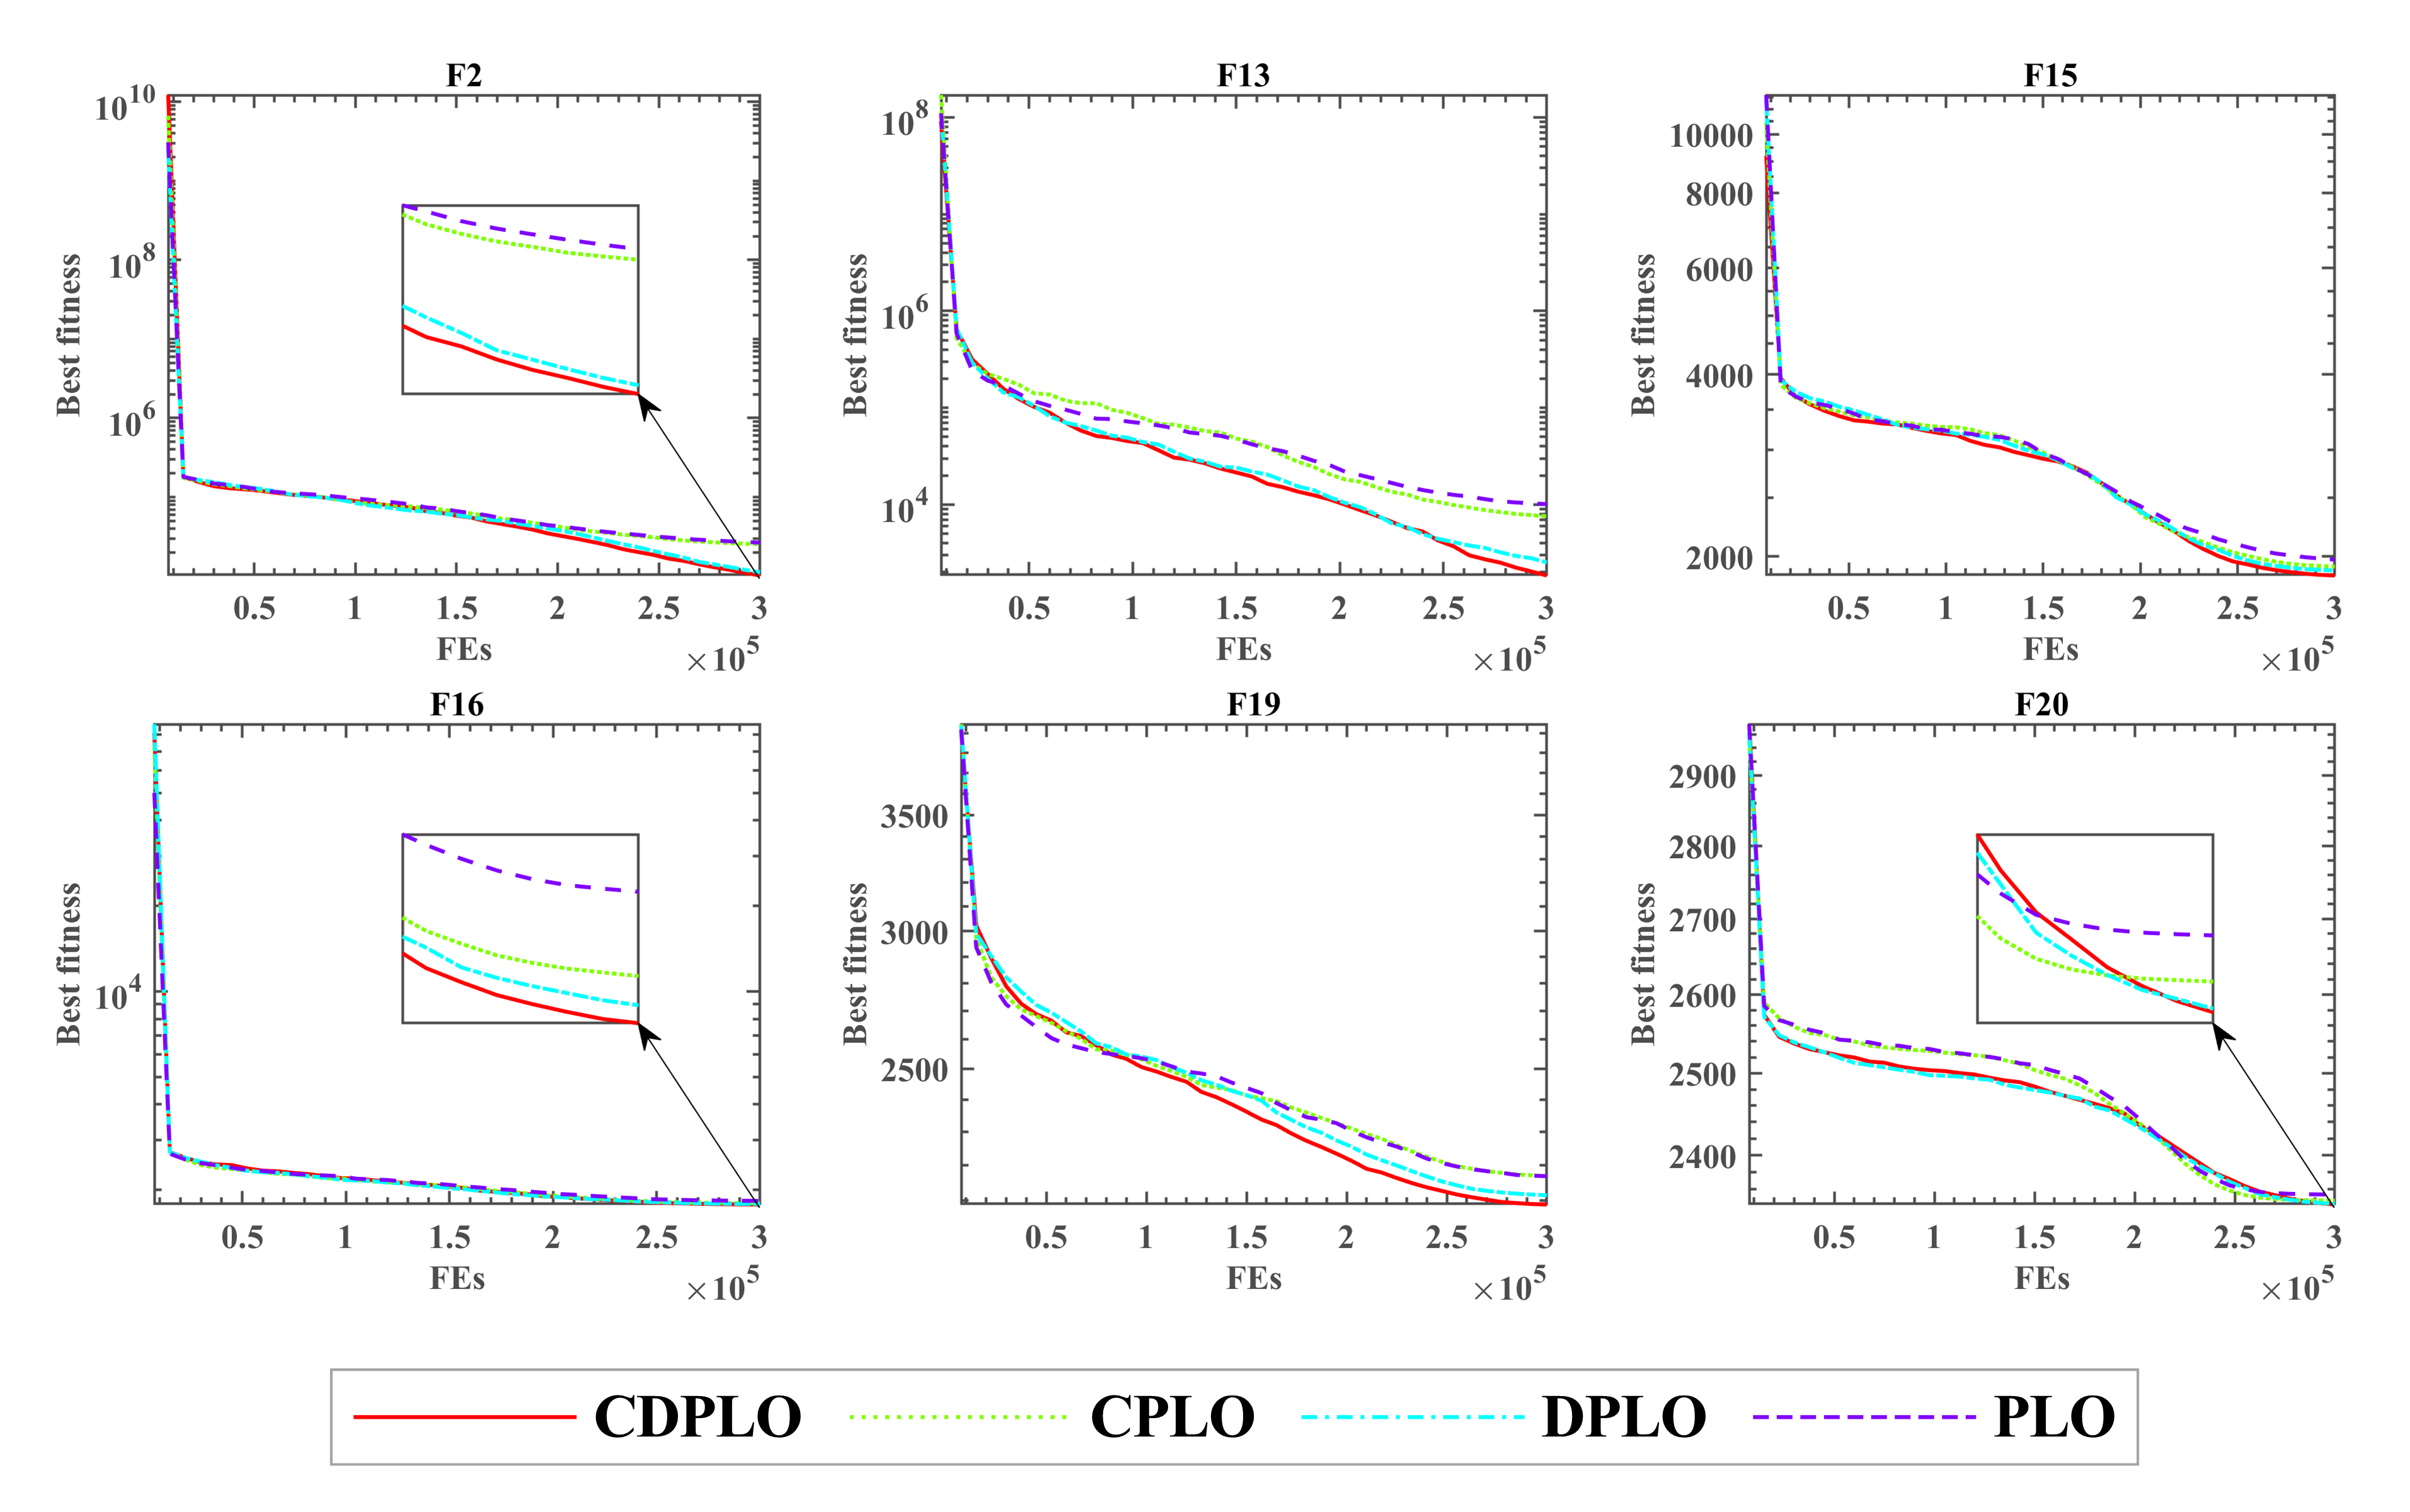
\includegraphics[width=\linewidth]{CDPLO-Ablation}
\label{fig: CDPLO-Ablation-CC}
\end{figure}

For a more comprehensive showing the robustness the algorithm in the test functions, we have visulized the 30 independent runs for those algorithm, since the fitness value may vary in a very long range, we have made the appropriate scale for the fitness value to better differentiate them while present the result in a decent way. The boxplot result are showin in Fig. \ref{fig: CDPLO-Ablation-boxplot}. The scatter dot and the relative fitness value can be seen in the figure, the lower the bar, the dense the scatter dots, the better the algorithm's robustness and performance. Obviously, the PLO shows the highest bar while a relative sparse scatter dots distribution, while the CPLO and DPLO both have a relative lower bar compare with the original PLO, the fusion of them CDPLO obtain the lowest bar height and the most dense scatter dots in total, represent better robustness and performance over other PLO variants and PLO algorithm. 

 \begin{figure}
\centering
\caption{Scaled best fitness (box-and-scatter) of the four
           methods over 30 runs on the same six functions.}
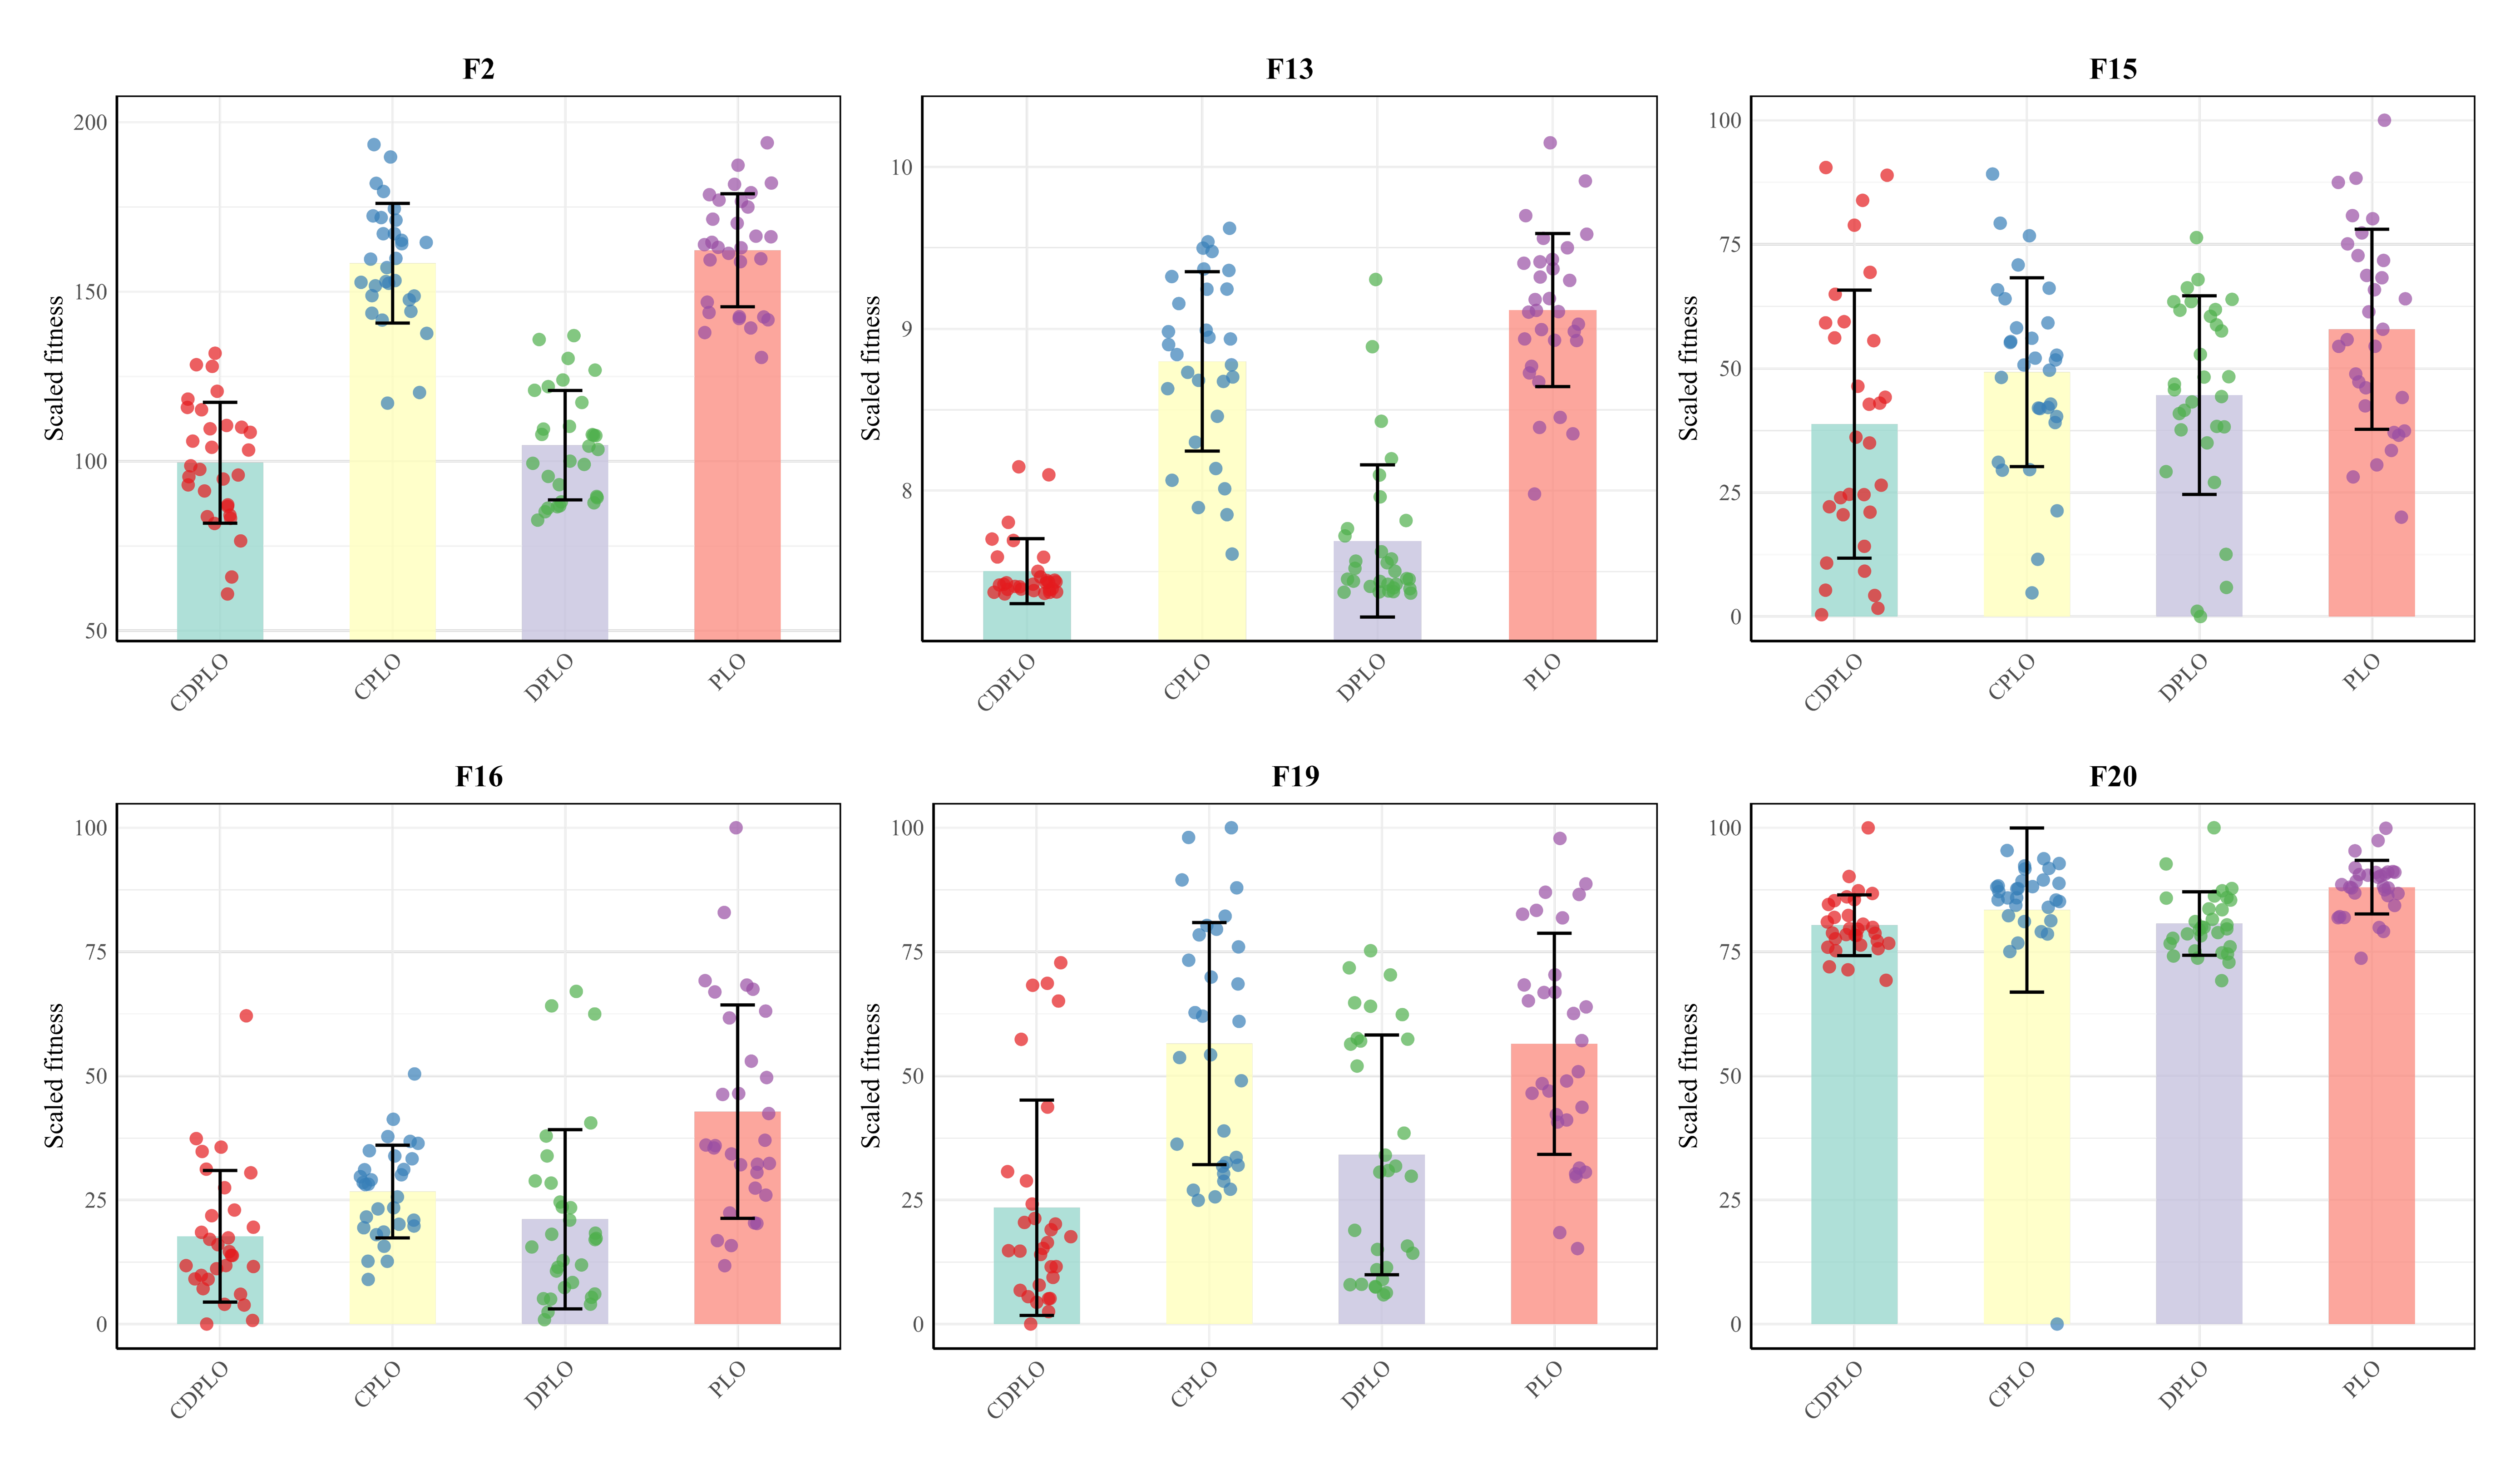
\includegraphics[width=\linewidth]{CDPLO-Ablation-boxplot}
\label{fig: CDPLO-Ablation-boxplot}
\end{figure}

For the sake of better seeing each algorightm performance over each 29 functions, we provide the radar plot in Fig. \ref{fig: Abation-FR}(a), assisted with a ARV and FR value bar plot in Fig. \ref{fig: Ablation-FR}(b).

\begin{figure}
\centering
\caption{Average-rank value (ARV) and Friedman post-hoc ranking
           of the four methods over all 30 CEC 2017 functions.}
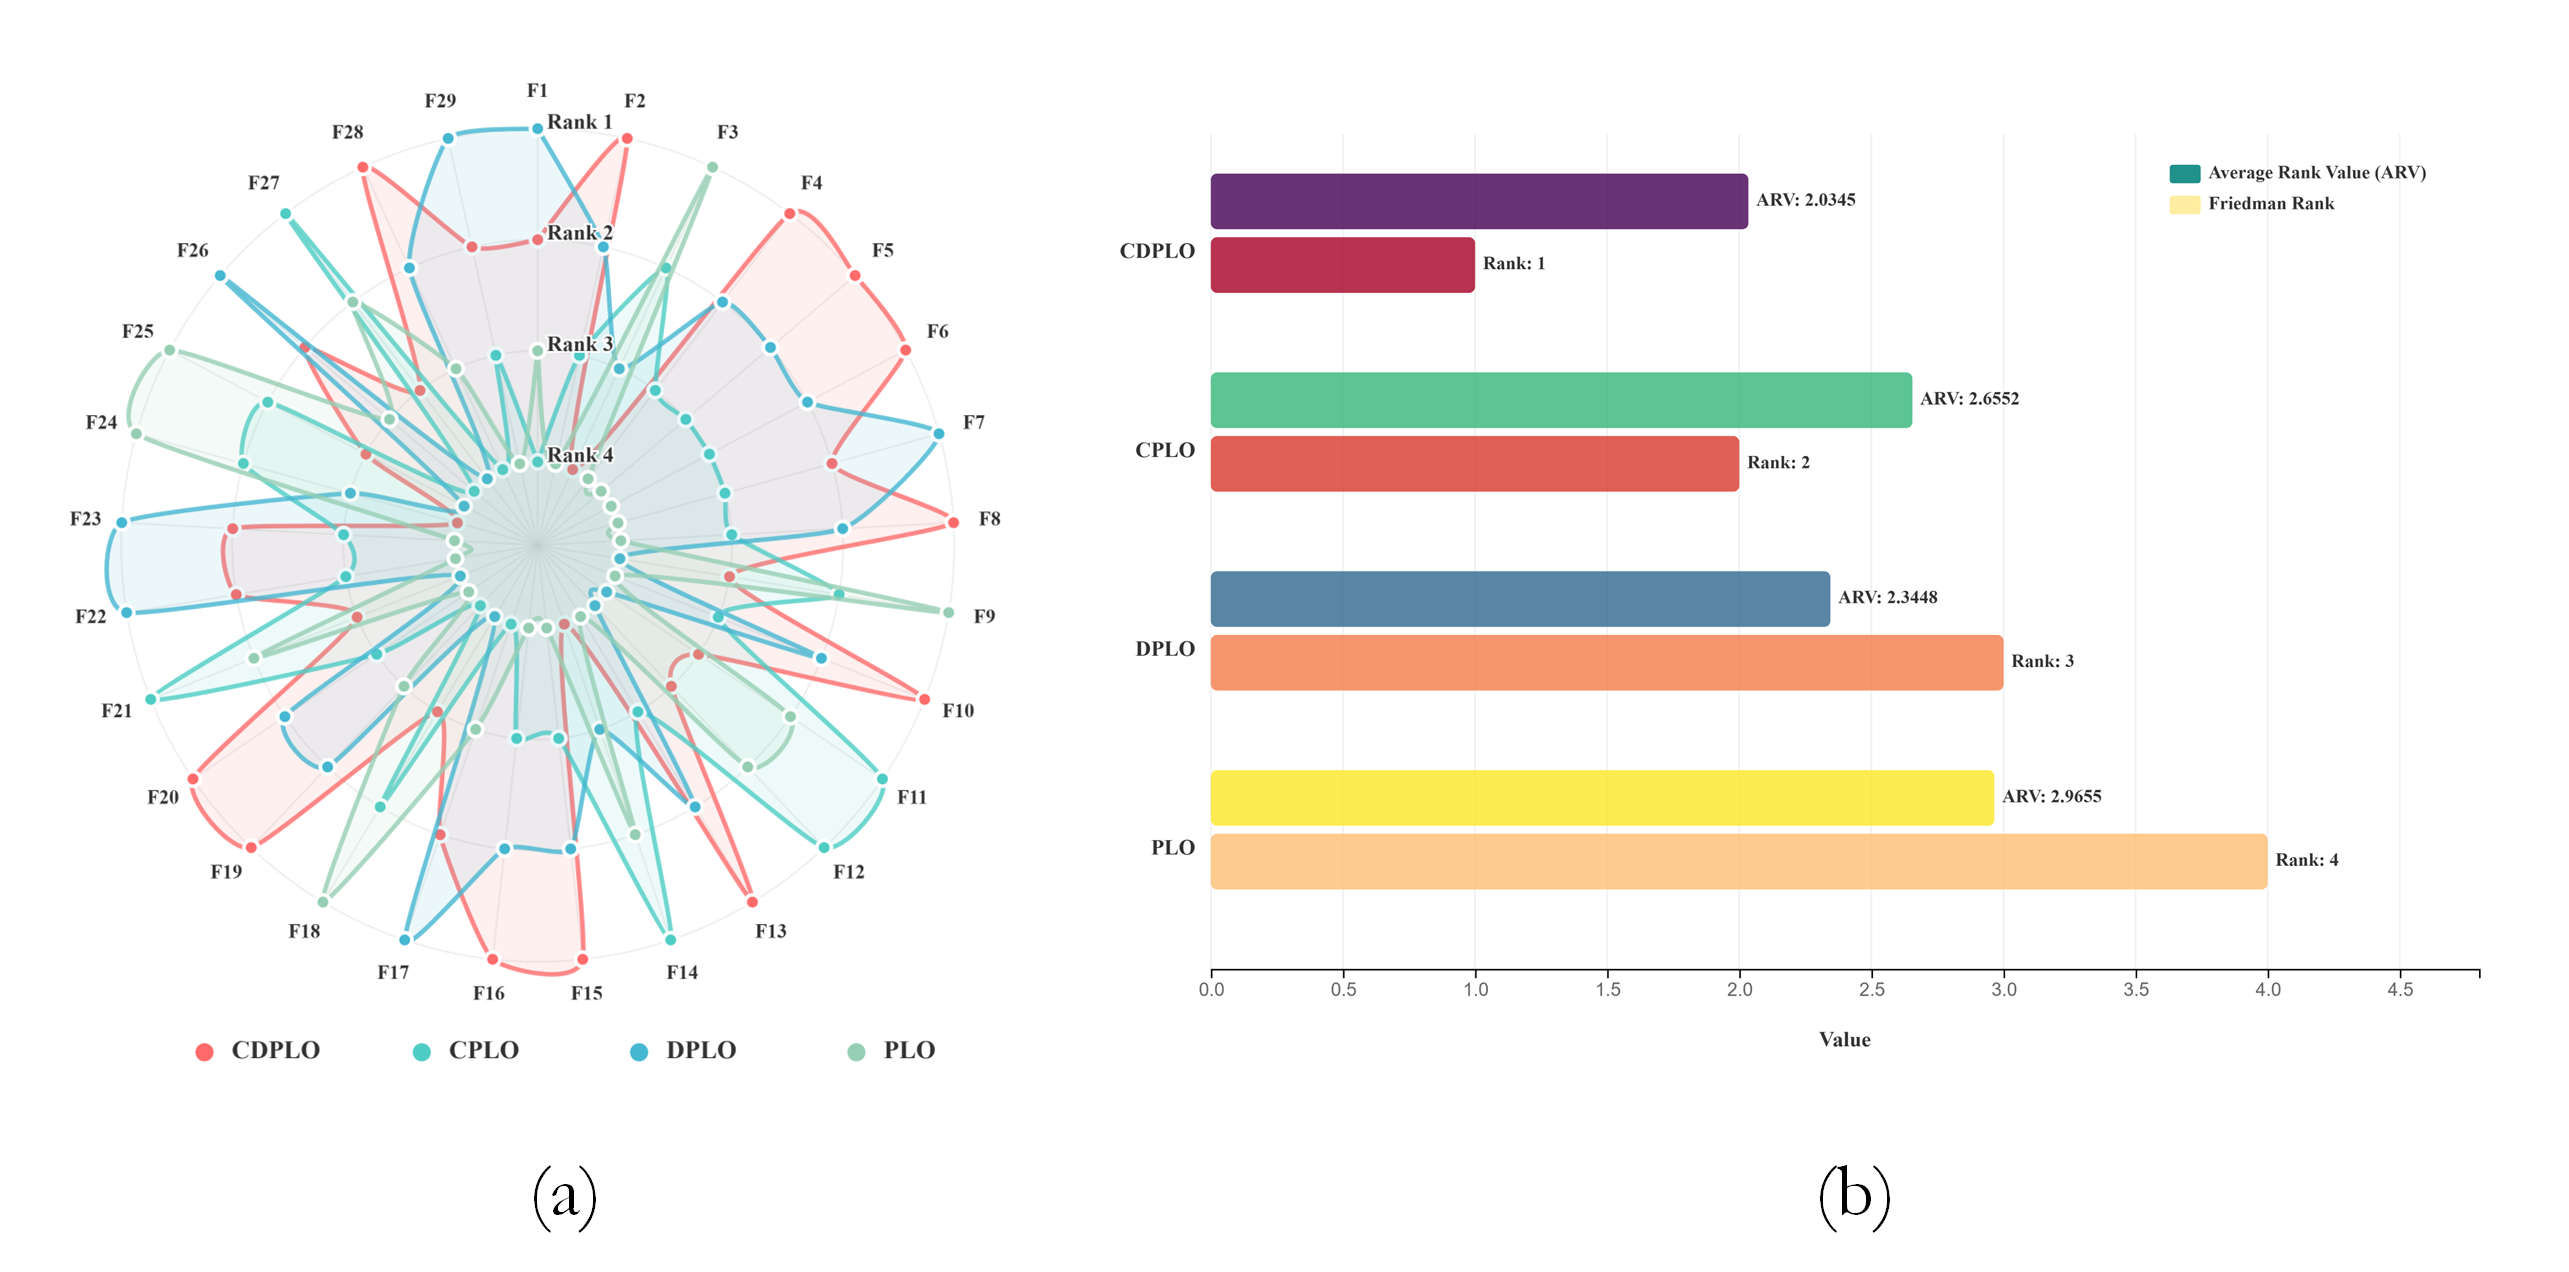
\includegraphics[width=\linewidth]{Ablation-FR}
\label{fig: Ablation-FR}
\end{figure}

\begin{table}
\centering
\caption{Comparison results of PLO and its variants.}
\label{table: CDPLO-Ablation}
\begin{tabular}{@{}lcccccccccccccccc@{}}
\end{tabular}
\end{table}

\subsection{Testing on IEEE CEC 2017}
% This section should show the statistic result and the convergence curve (compare with 9 optimizer)
To comprehensive benchmark the performance of the proposed CDPLO performance, we compare it with 9 state-of-the-art optimization method proposed recently. Black-winged Kite Algorithm (BKA) \ref{}, Status-Based Optimization (SBO) \ref{}, IVY algorithm (IVY) \ref{}, Cross Aaptive Grey Wolf Optimization (CAGWO) \ref{}, Roulette wheel and Mutation improved RIME (RMRIME) \ref{}, Slime Mould Algorithm incorporating Differential Evolution and Powell mechanism (PSMADE) \ref{}, Double adaptive Random spare reinforced Whale Optimization Algorithm (RDWOA) \ref{}, Elite Opposition-Based Learning mutation enhanced Sparrow Search Algorithm (EOBLSSA) \ref{}, Generalized Oppositional Teaching Learning Based Optimization (GOTLBO) \ref{}. We present the comparison results in Table \ref{table: CDPLO-Cmp}, with the best results bolded for better recognization. Also, the non-parametric statistic analysis are included in the last three columns of the table, including the WSRT result, the ARV result and the FR result. The result indicate the proposed CDPLO have a comparative performance among all the peers compared.

We select six functions to visualize the comparison result, the convergence curves are presented in the Fig. \ref{fig: CDPLO-Cmp}, the selected functions are multimodal functions F5 and F8, hybrid functions F15 and F19, composite functions F23 and F25. Due to the inherent overly diversity population of the PLO algorithm, the proposed CDPLO algorithm did not show the fastest convergence curves in the plots, while the introduction of the cluster guidance and the differential recombination, the escape local optima ability of CDPLO and the solution quality had been greatly refined. So although the convergence curves is not so fast in showing in the plot, the solution quality is indeed very comparitive compare with the peers.

\begin{figure}
\caption{Convergence behaviour of CDPLO versus nine
           competitors on six representative CEC 2017 functions.}
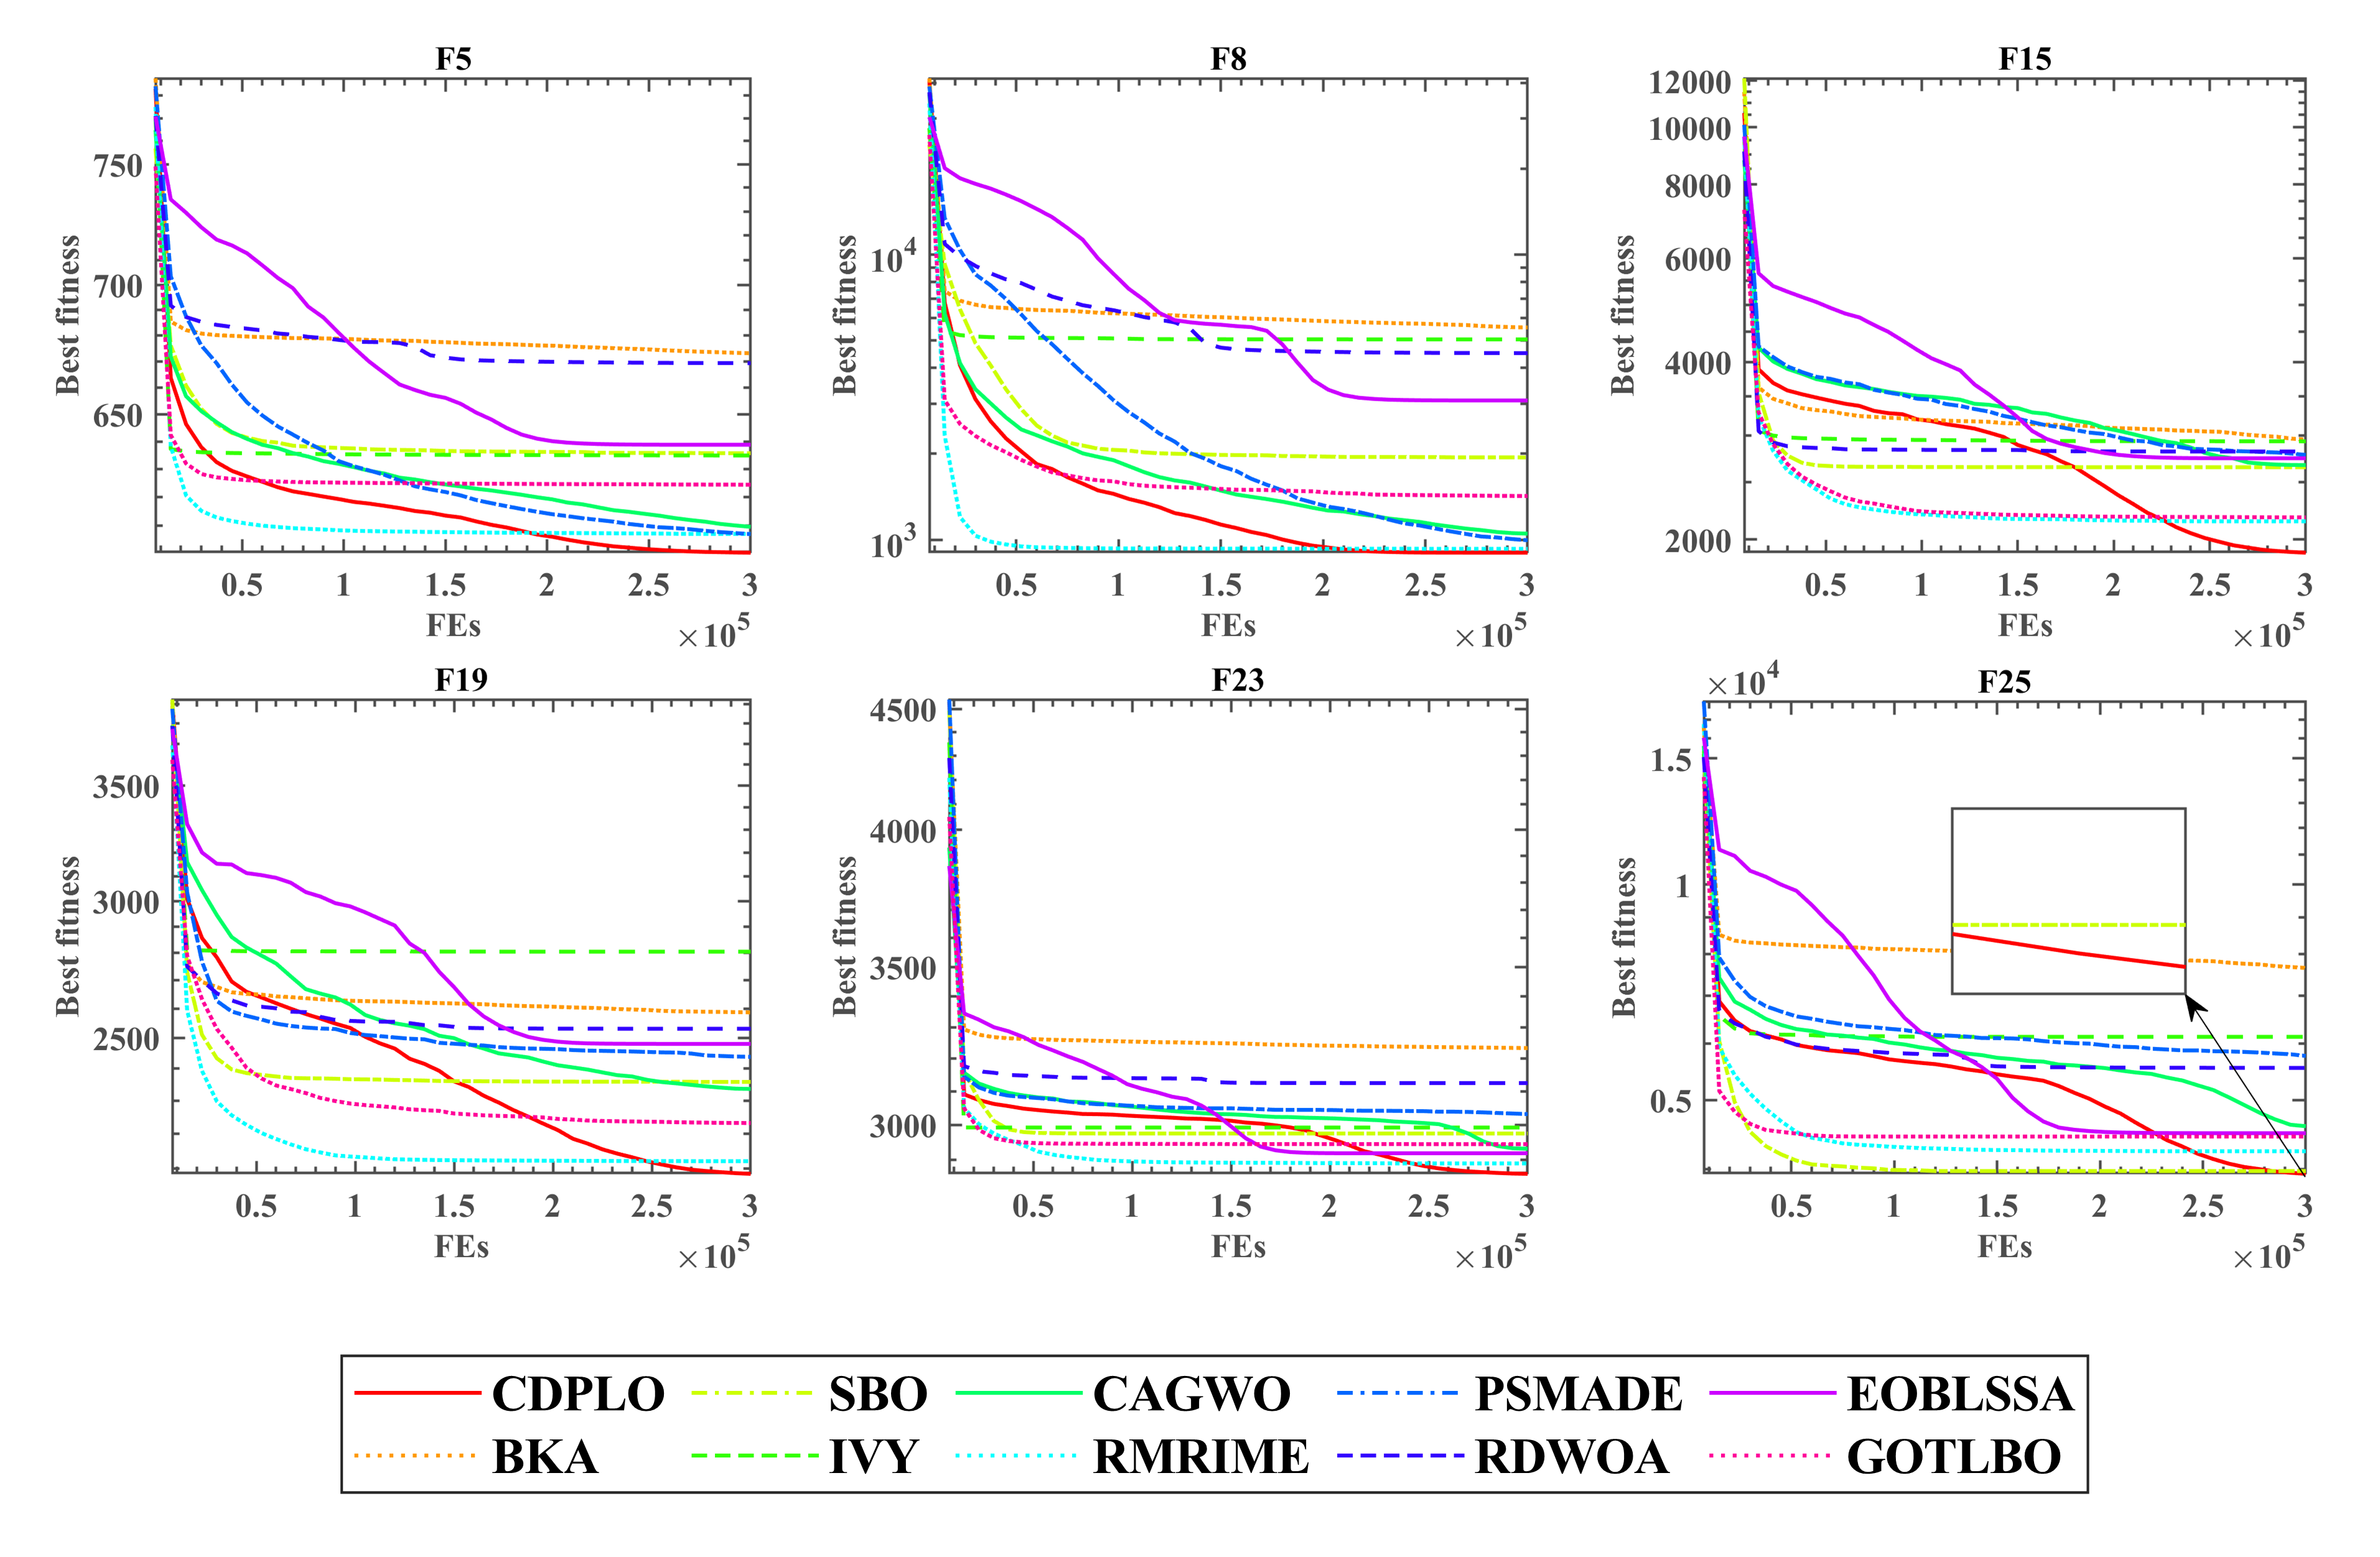
\includegraphics[width=\linewidth]{CDPLO-Cmp}
\label{fig: CDPLO-Cmp}
\end{figure}

Besides, we provide the scatter dots of 30 independent runs of those algorithm and their relative average fitness on selected functions to differentiate their variability during optimization. The plots are presented in the Fig. \ref{CDPLO-Cmp-boxplot}, we can seen that the proposed CDPLO obtain the densest dots in the plots, and the lowest fitness value compare with the peers. This shows the strong robustness of the proposed CDPLO algorithm and its performance. Also, we visulize those algorithm in each of the CEC 2017 functions rank in a radar plot in Fig. \ref{Cmp-FR}(a), and the FR result and AVR result in Fig. \ref{Cmp-FR}(b). Seen from those two figures, the CDPLO have otained the most first rank in the radar plot while shows the lowest FR value and ARV value in the bar plot. Those results strongly indicate the proposed CDPLO have relative superior performance to the peers. For further showing the CDPLO's ability in real-world application, we conducted a feature selection task for preeclampsia prediction.

\begin{figure}
\caption{Scaled best fitness (box-and-scatter) for the ten
           algorithms.}
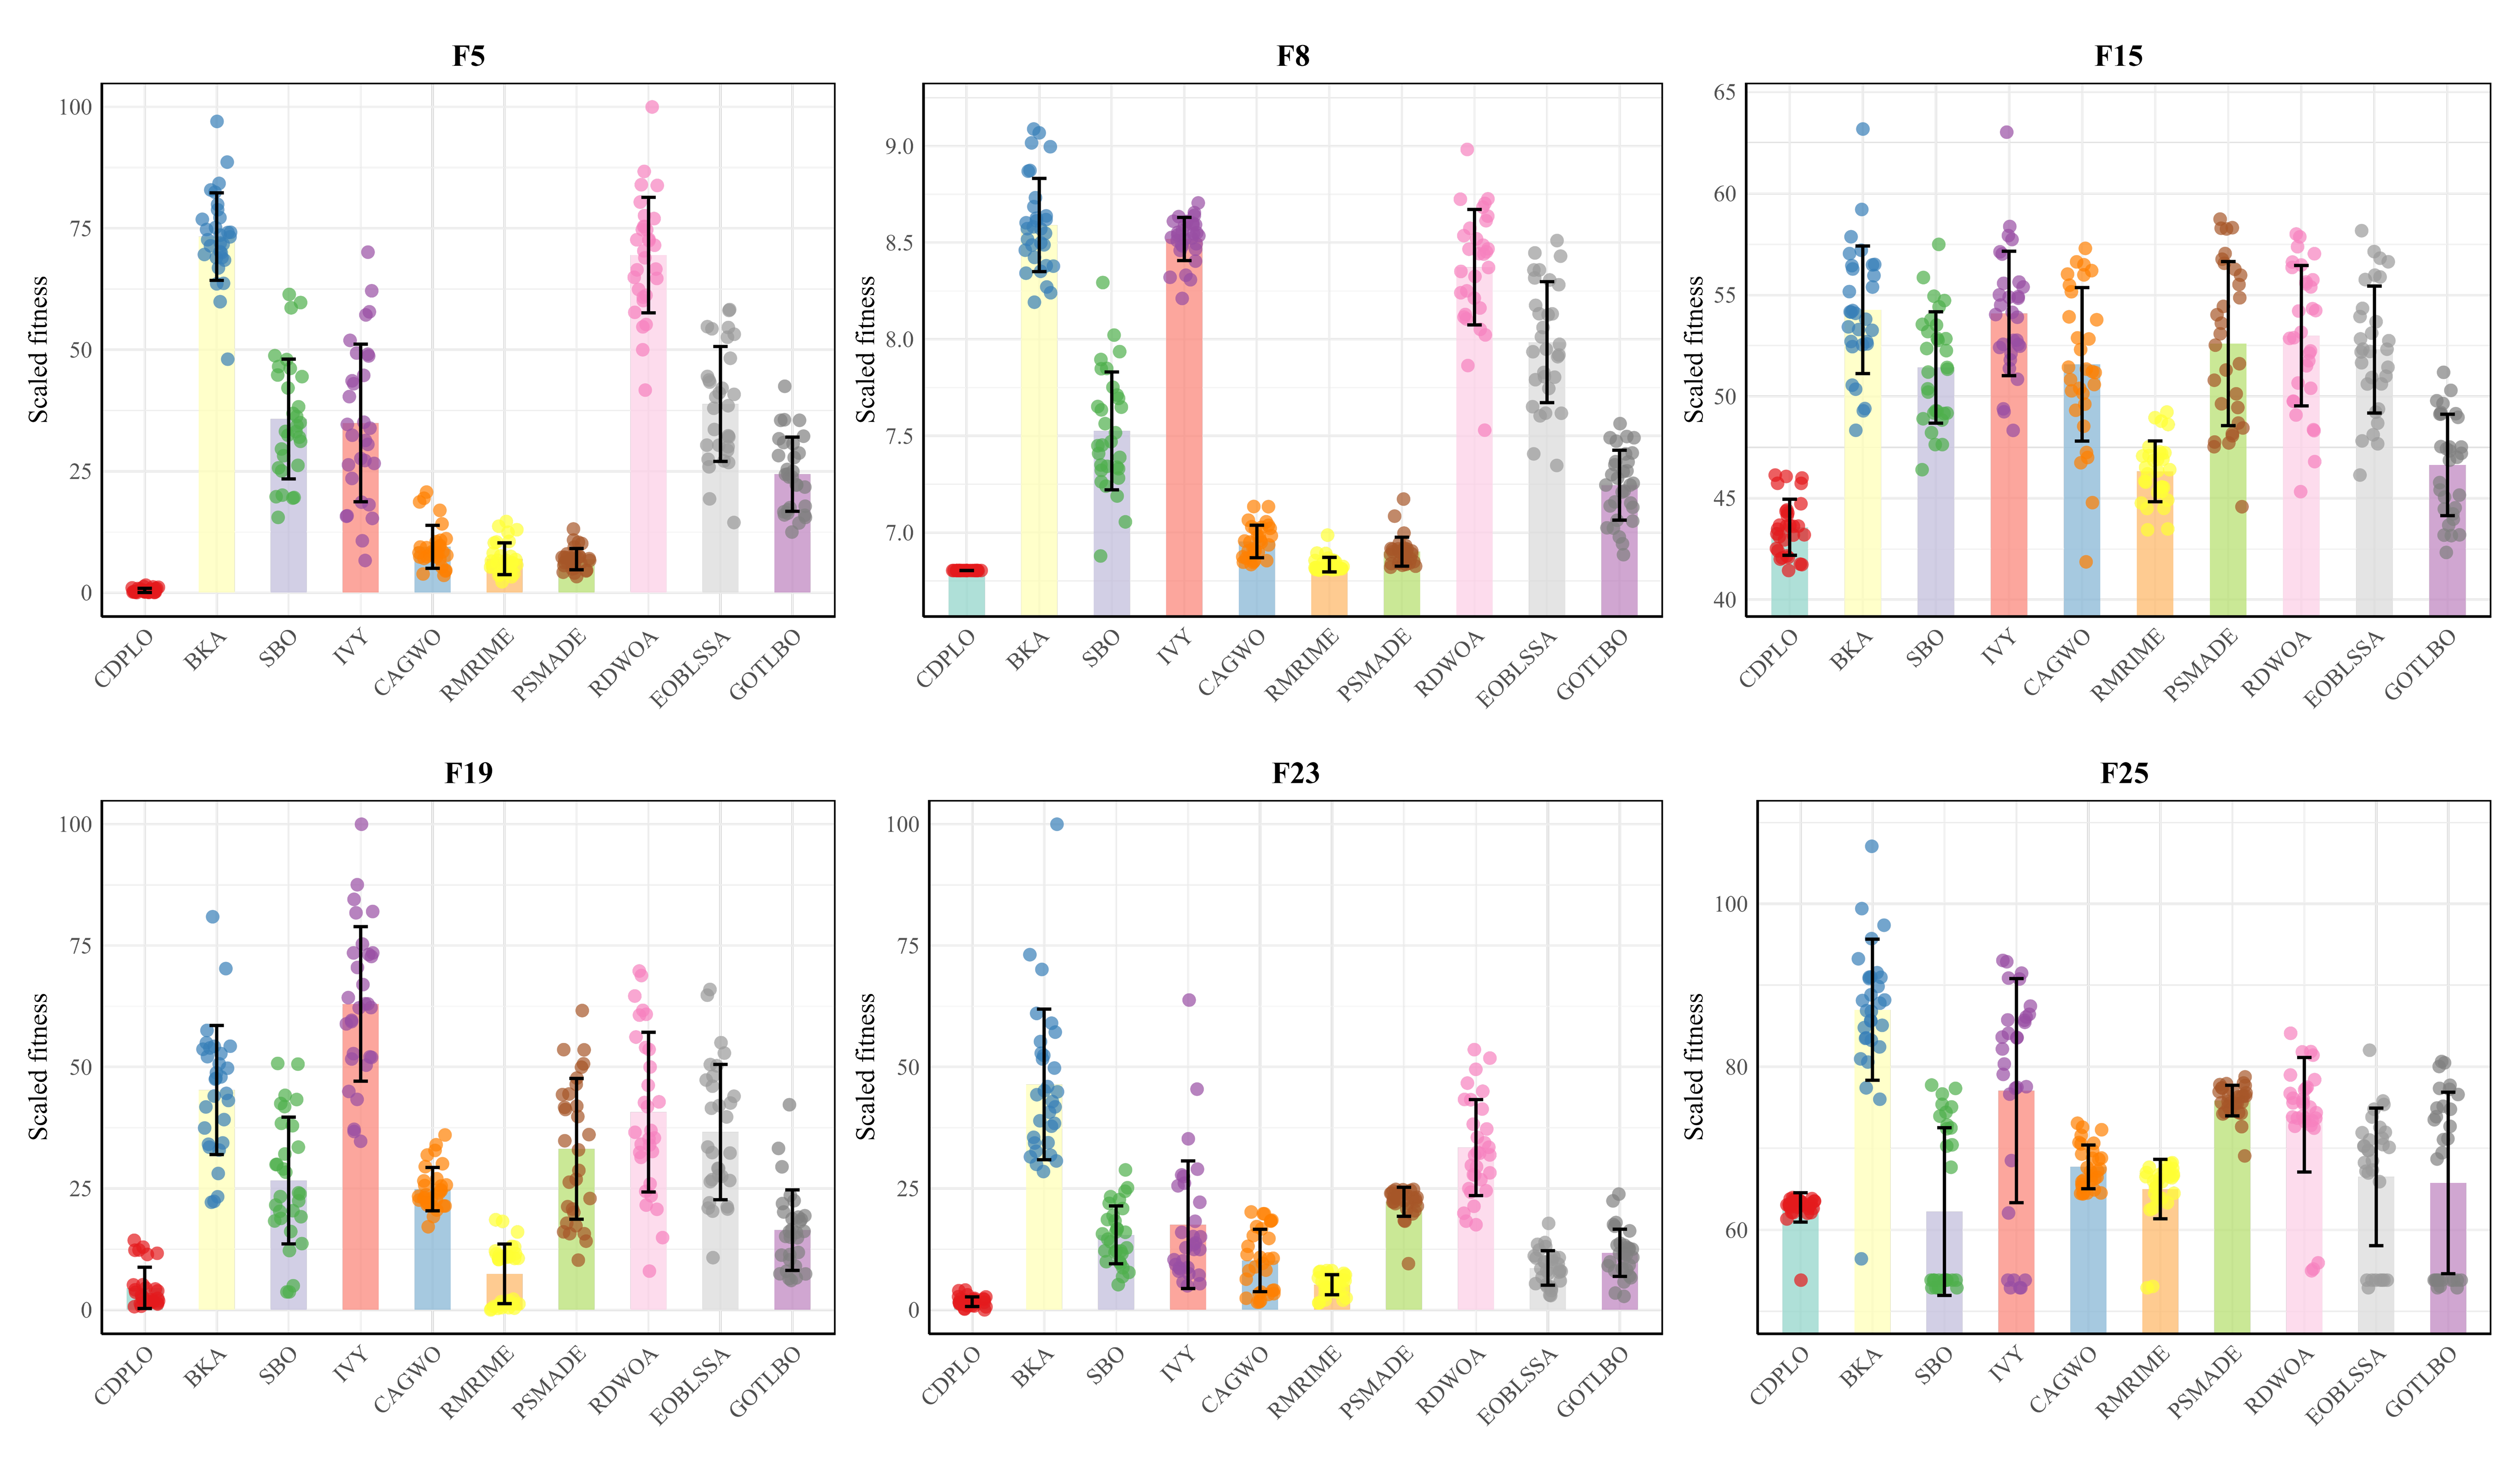
\includegraphics[width=\linewidth]{CDPLO-Cmp-boxplot}
\label{fig: CDPLO-Cmp-boxplot}
\end{figure}

\begin{figure}
\caption{Global ranking on the full 30-function suite:
average-rank value and Friedman test.}
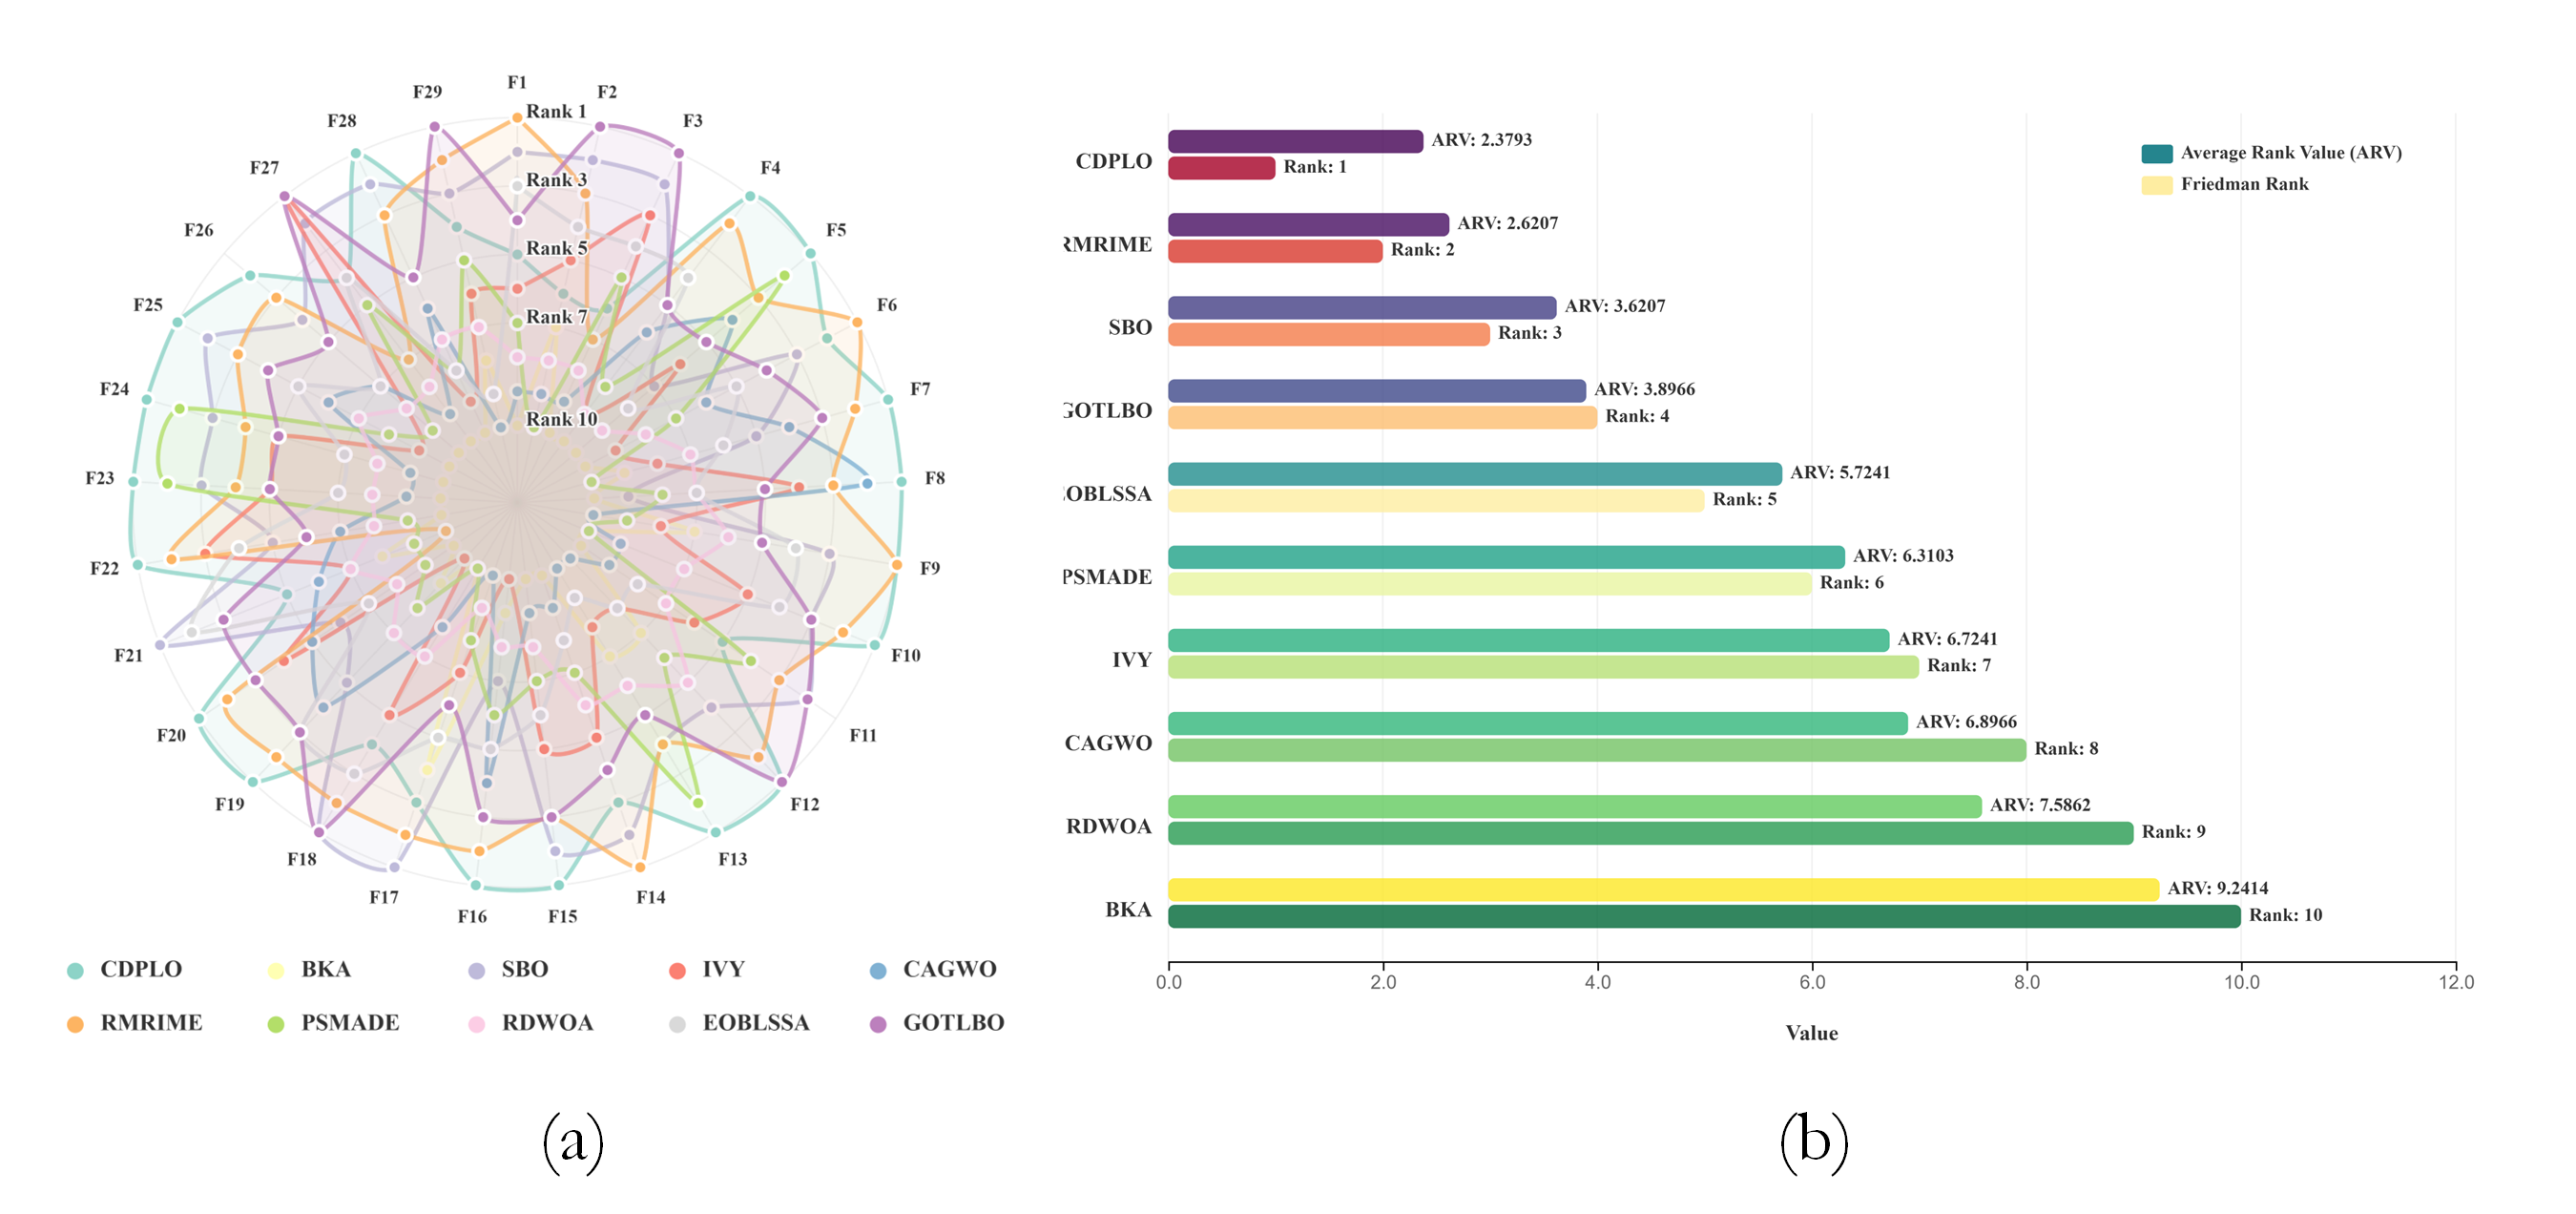
\includegraphics[width=\linewidth]{Cmp-FR}
\label{fig: Cmp-FR}
\end{figure}

\begin{table}
\centering
\begin{tabular}{@{} lcccccccccccccccc @{}}
\end{tabular}
\end{table}

\bibliography{PLOJF}

\end{document}
